\documentclass[11pt, oneside]{article}   	% use "amsart" instead of "article" for AMSLaTeX format
\usepackage{geometry}                		% See geometry.pdf to learn the layout options. There are lots.
\geometry{letterpaper}                   		% ... or a4paper or a5paper or ... 
%\geometry{landscape}                		% Activate for for rotated page geometry
%\usepackage[parfill]{parskip}    		% Activate to begin paragraphs with an empty line rather than an indent
\usepackage{graphicx}				% Use pdf, png, jpg, or eps§ with pdflatex; use eps in DVI mode
								% TeX will automatically convert eps --> pdf in pdflatex		
\usepackage{amssymb}
\usepackage{bm}
\usepackage{natbib}
\usepackage{subfig}

\title{Conditional Ground Motion Simulations in ShakeMap}
\author{Nick Horspool, Bruce Worden & David Wald}
%\date{}							% Activate to display a given date or no date

\begin{document}
\maketitle

\section{Introduction}

This document outlines the method of generating ground motion fields with spatially correlated residuals that are conditional on observed ground motions within the ShakeMap framework. \\

At present, ShakeMap produces maps of median ground motions and uncertainty. If the estimated ground motions are to be used to assess potential damage and loss for an independent building then the current outputs are sufficient.  However, if an assessment of the damage and loss to a portfolio of buildings or a distributed network is required it is critical to consider the correlation of loss to all assets in the portfolio or network. \\

ShakeMap removes inter-event variability through bias correction of the GMPE, with the remaining uncertainty due to intra-event uncertainty of the GMPE, or from an unknown source geometry. When considering losses to a portfolio, the spatial correlation of the intra-event uncertainty must be taken into account. Work by \citet{park2007} have shown that not accounting for spatial correlation of intra-event uncertainty will significantly underestimate the losses, as spatial correlation allows areas of high residuals to occur and at some occurrence these will be located in the areas of highest exposure. To account for the spatial correlation of intra-event uncertainty, a simulation approach is required. Where a number of ground motion fields are generated that each represent a possible realisation of the spatially correlated residuals. 

This document outlines the general method for how this can be accomplished using the existing ShakeMap framework. 

\section{Work Flow}

Ground motion prediction equation. 

\begin{equation}
log(Y_{ij}) = \overline{log Y_{ij}} (M_i, R_{ij}, \theta_{i1,i2,...,iN} ) + \tau \eta_i + \sigma \varepsilon_{ij}
\label{eq_gmpe}
\end{equation}

where $Y_{ij}$ is the ground motion intensity measure at site $j$ during earthquake $i$, and log $Y_{ij}$ is the median of the log of Y for an earthquake with magnitude $M_i$ at distance $R_{ij}$, and $\theta{i1,i2,...,iN}$ are additional variables that describes earthquake source, path or site effects. The uncertainty in the ground motion intensity measure is partitioned into inter-event ($\tau \eta_i$) and intra-event ($\sigma \varepsilon_{ij}$) error terms or also referred to as residuals. $\tau$ and $\varepsilon_{ij}$ are normally distributed errors with mean of zero and standard deviation of one. $\eta_i$ and $\sigma$ are the standard deviations of the respective error terms defined by the ground motion prediction equation.

For a given earthquake, $i$, the inter-event error term, $\tau \eta_i$, is consistent across all sites, where as the intra-event error, $\sigma \varepsilon_{ij}$, varies from site to site. It has been shown that the intra-event error term, $\varepsilon_{ij}$, $\varepsilon_{ik}$ between two sites $j$ and $k$ is spatially correlated. Folllowing work used observed ground motions from well recorded earthquakes with dense networks to develop empirical correlation models for $\varepsilon_{ij}$ (e.g. GH 2008, JB 2009, LB 2013). 

If the intra-event error term is spatially correlated then this must be accounted for when generating ground motion field simulations, both in a predictive mode when a future earthquake is being modelled, as well as for an earthquake that has already occurred. In the case of the latter, ground motion fields can be generated that are conditional on the observed ground motions. 

The empirical spatial correlation function is defined as:
\begin{equation}
\rho_{ij} (T)= 1 - e^{-3h/b(T)}
\label(eq_cor}
\end{equation}

where $h$ is the distance between two sites, $i$ and $j$, and $b$ is defined as the correlation length, or range. Empirical models for $b$ as a function of period $T$ have also been defined:

\begin{equation}
b(T) = d_1 + d_2T
\end{equation}

where $d_1=11.7$ and $d_2=12.7$.

\subsection{Generation of unconditional spatially correlated ground motion fields (no observed data)}

In the case where no observed ground motions are available, for example when modelling a scenario earthquake or an earthquake that has already occurred but has no observed data, the following approach of  \cite{park2007} is adopted.  We aim to generate a vector of correlated, normally distributed random variables:

\begin{equation}
\bm{X} = \Big [ X_1, X_2,...,X_M \Big ]
\end{equation}

where $X_j = \varepsilon_{ij}$ is the residual term from equation \ref{eq_gmpe}. $\bm{X}$ is defined by a covariance matrix ($\Sigma$), or in shorthand $X \sim N_M(\bm{0}, \Sigma)$, which has dimension $k$ x $l$ and defines the covariance between the $k^{th}$ and $l^{th}$ sites which is calculated using equation \ref{eq_cor} where $h$ is the distance between the sites $k$ and $l$. 

In the case of no observed data, the vector of spatially correlated random normal variates, $\bm{X}$, can be calculated by:

\begin{equation}
 \bm{X}=\bm{AU}$
 \label{eq_X}
 \end{equation}
 
 where
 
\begin{equation}
\bm{U} = \Big [ \bm{U_1}, \bm{U_2},...,\bm{U_M} \Big ]
\end{equation}

is a vector of random normal variables with mean of zero and standard deviation of one, and $\bm{A}$ is the lower triangular matrix generated from a Cholesky decomposition of the covariance matrix $\Sigma$ such that

\begin{equation}
\bm{AA^T} = \Sigma
\end{equation}

Once the vector of spatially correlated intra-event residuals, $\bm{X}=\varepsilon_{ij}$ has been calculated, these values can be added to the back to the median ground motion, $log(Y_{ij})$, to create a single ground motion field realisation. In practise, a number of realisations should be calculated by regenerating the vector $\bm{U}$ and reevaluating equation \ref{eq_X}.

\subsection{Generation of conditional spatially correlated ground motion fields (with observed data)}


In the case where observed data is available for an event that has already occurred, the method here follows that of \citet{park2007}. The aim is still to define $X$, but in this case, we have $X_{MOD}$ and $X_{OBS}$ for the modelled and observed sites. 

\begin{equation}
\Bigg [ \frac{\bm{X_{obs}} }{\bm{X'}} \Bigg ] \sim N_m \Bigg( \Bigg [ \frac{\bm{0}}{\bm{0}} \Bigg] , \Bigg[  \begin{array}{c|c}
  \bm{\Sigma_{11} } & \bm{\Sigma_{12}} \\
  \hline
  \bm{\Sigma_{21}} & \bm{\Sigma_{22}}
 \end{array} \Bigg]  \Bigg)
\end{equation}

\begin{equation}
\Big [ \bm{X'} \mid \bm{X_{obs}} =  \bm{x} \Big ] \sim N_m \Big (  \Big [   \bm{\Sigma_{21}} \bm{\Sigma_{11}^{-1}} \bm{x} \Big ] , \Big [  \bm{\Sigma_{22}} -  \bm{\Sigma_{21}} \bm{\Sigma_{11}^{-1}} \bm{\Sigma_{12}} \Big ] \Big)
\end{equation}

\begin{figure}
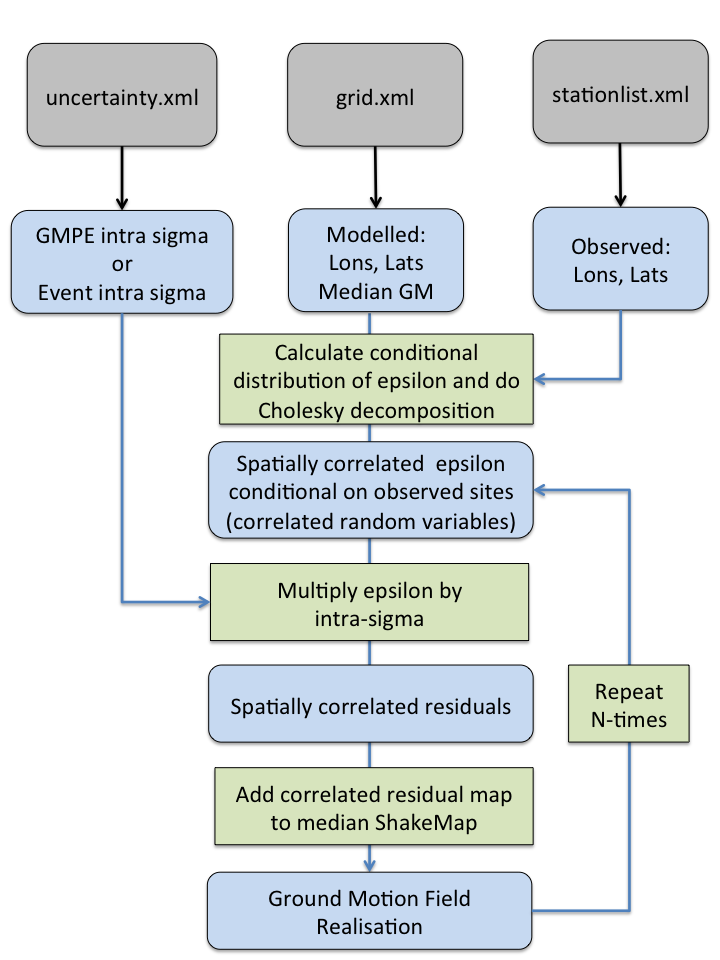
\includegraphics[width = 6in]{workflow.png}
\caption{Workflow for generating conditional ground motion simulations with ShakeMap}
\end{figure}

\begin{figure}
\subfloat[a]{\includegraphics[width = 3.5in]{test_csim_simulated_logresiduals.png}} \\
\subfloat[b]{\includegraphics[width = 3.5in]{test_csim_median_motions.png}}\\
\subfloat[c]{\includegraphics[width = 3.5in]{test_csim_simulated_motions.png}}
\caption{Steps in generating conditional ground motion simulations. A) Spatially correlated epsilon conditional on observed sites. This should be zero at observed sites B) Median ShakeMap C) Final conditional simulation map}
\label{steps}
\end{figure}

\begin{figure}
\subfloat[a]{\includegraphics[width = 3in]{GMF_medians.png}} 
\subfloat[b]{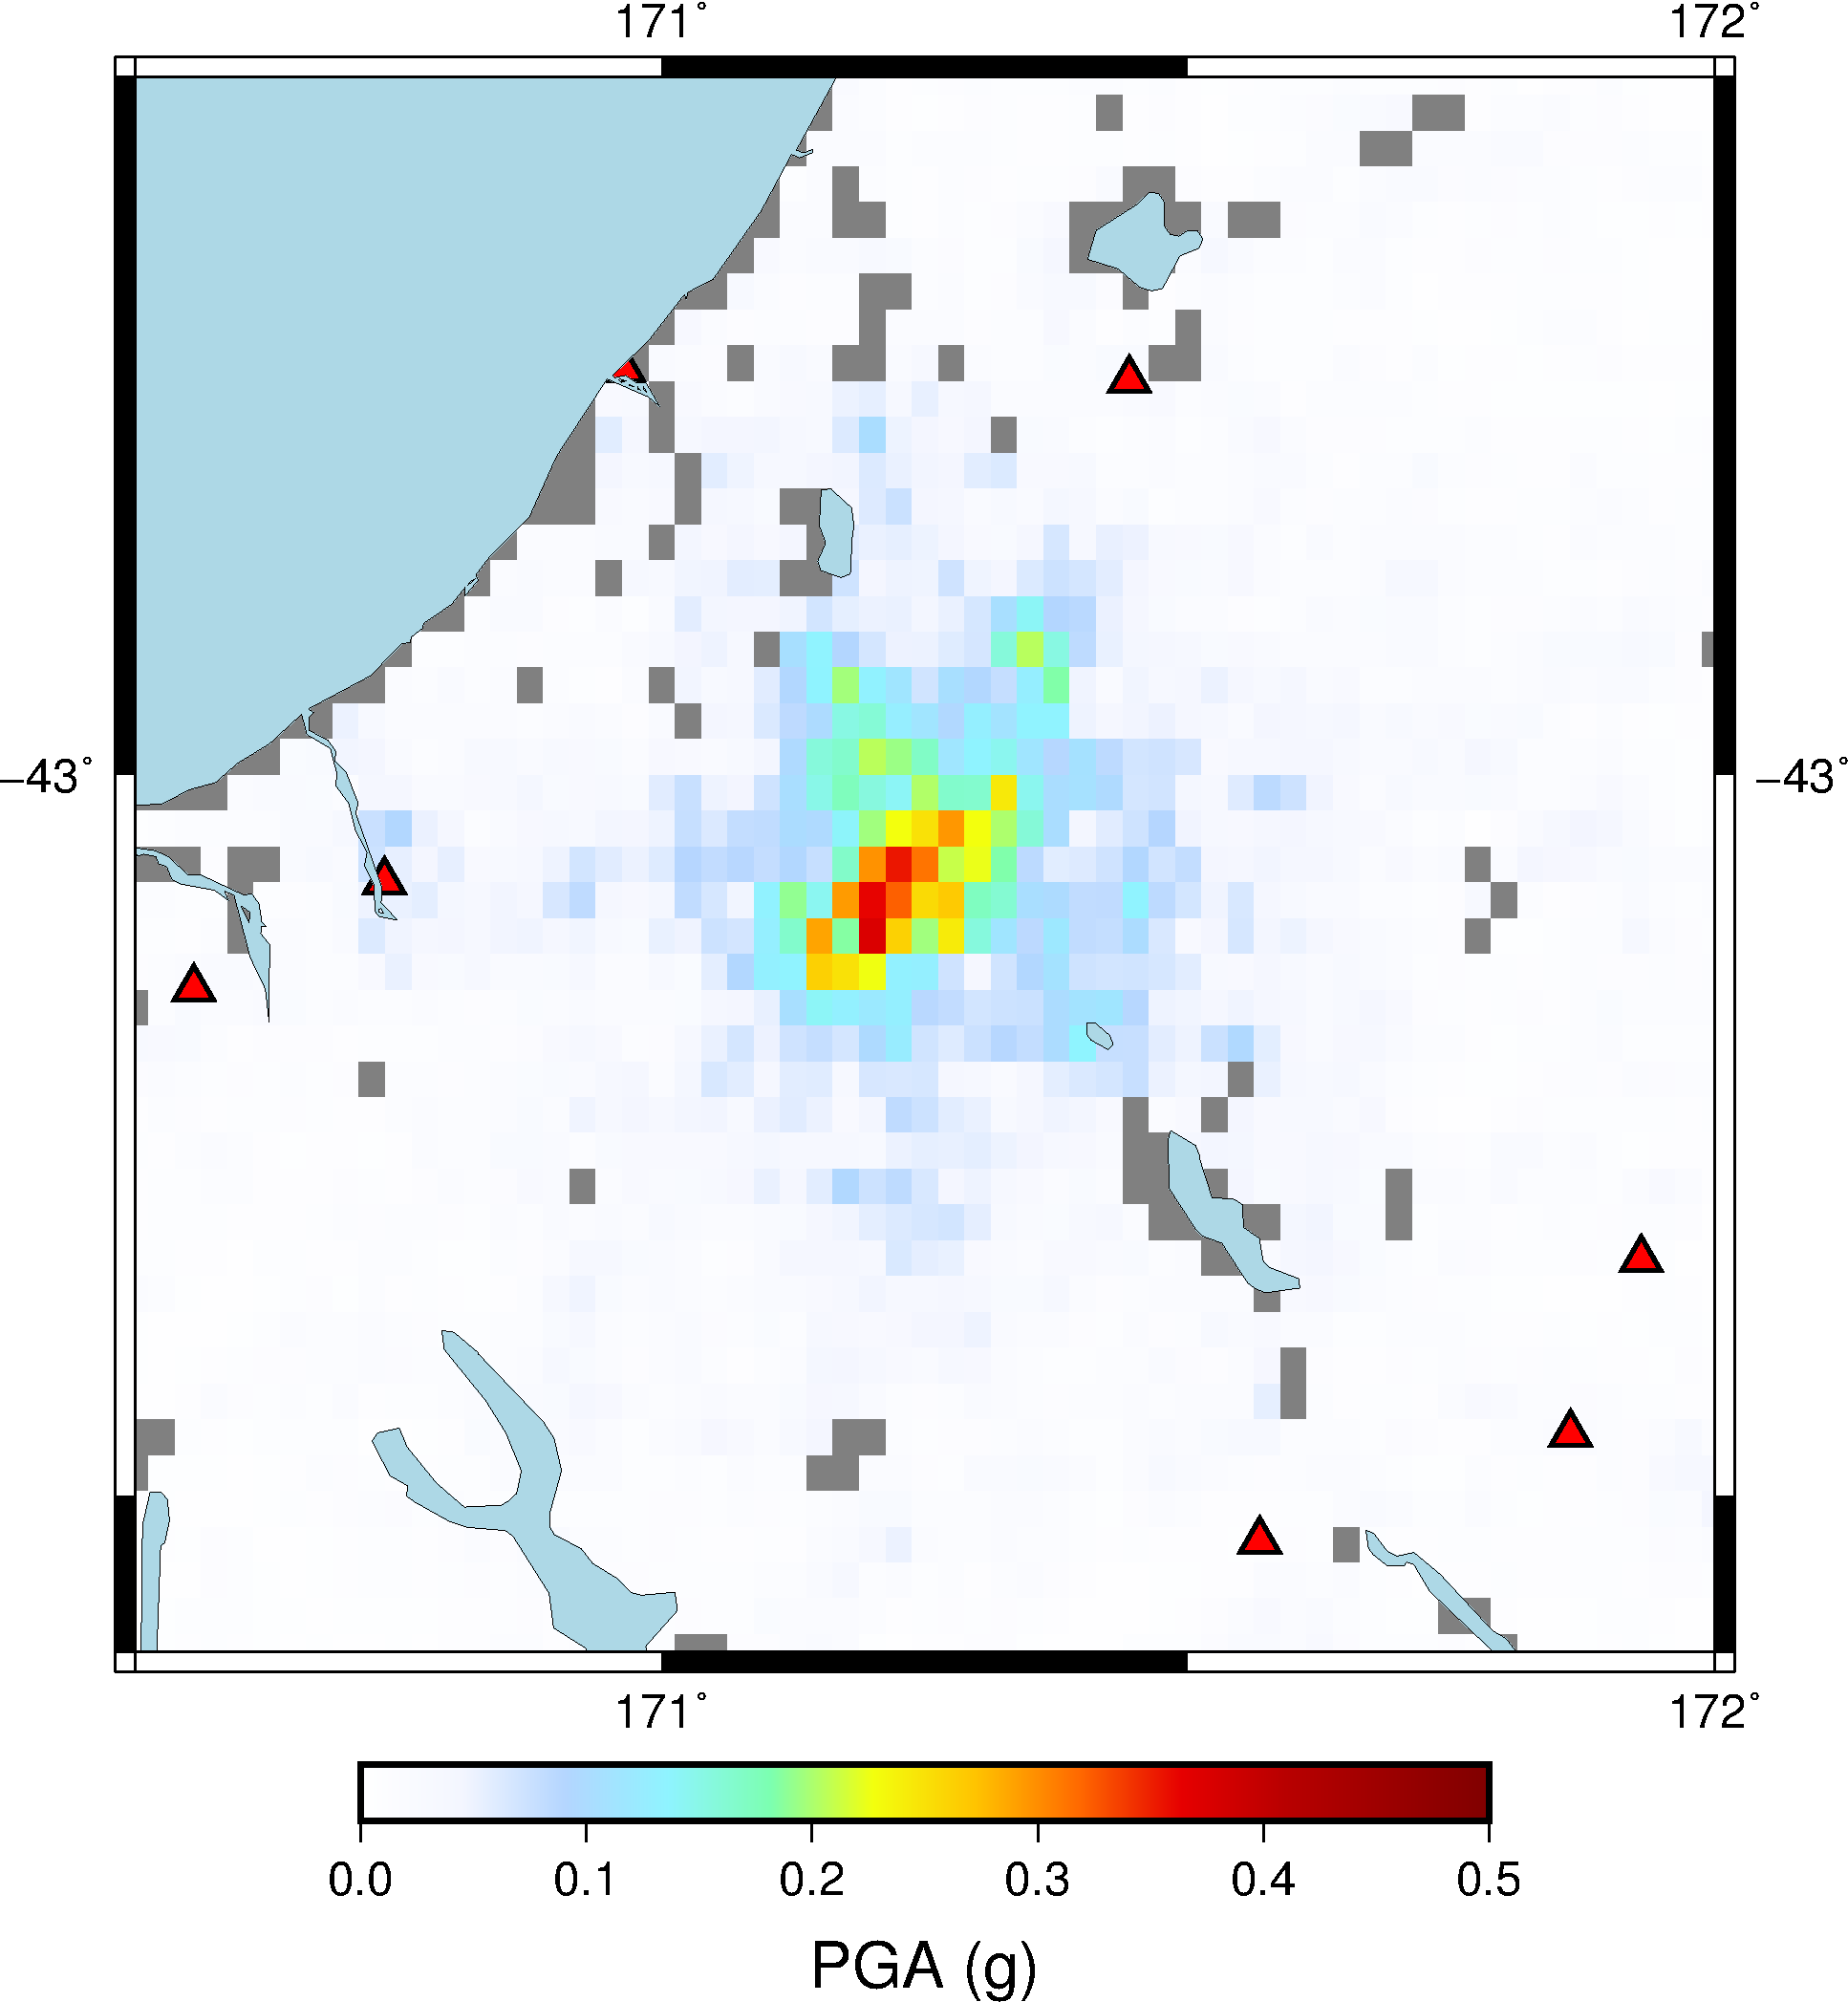
\includegraphics[width = 3in]{GMF_1.png}}\\
\subfloat[c]{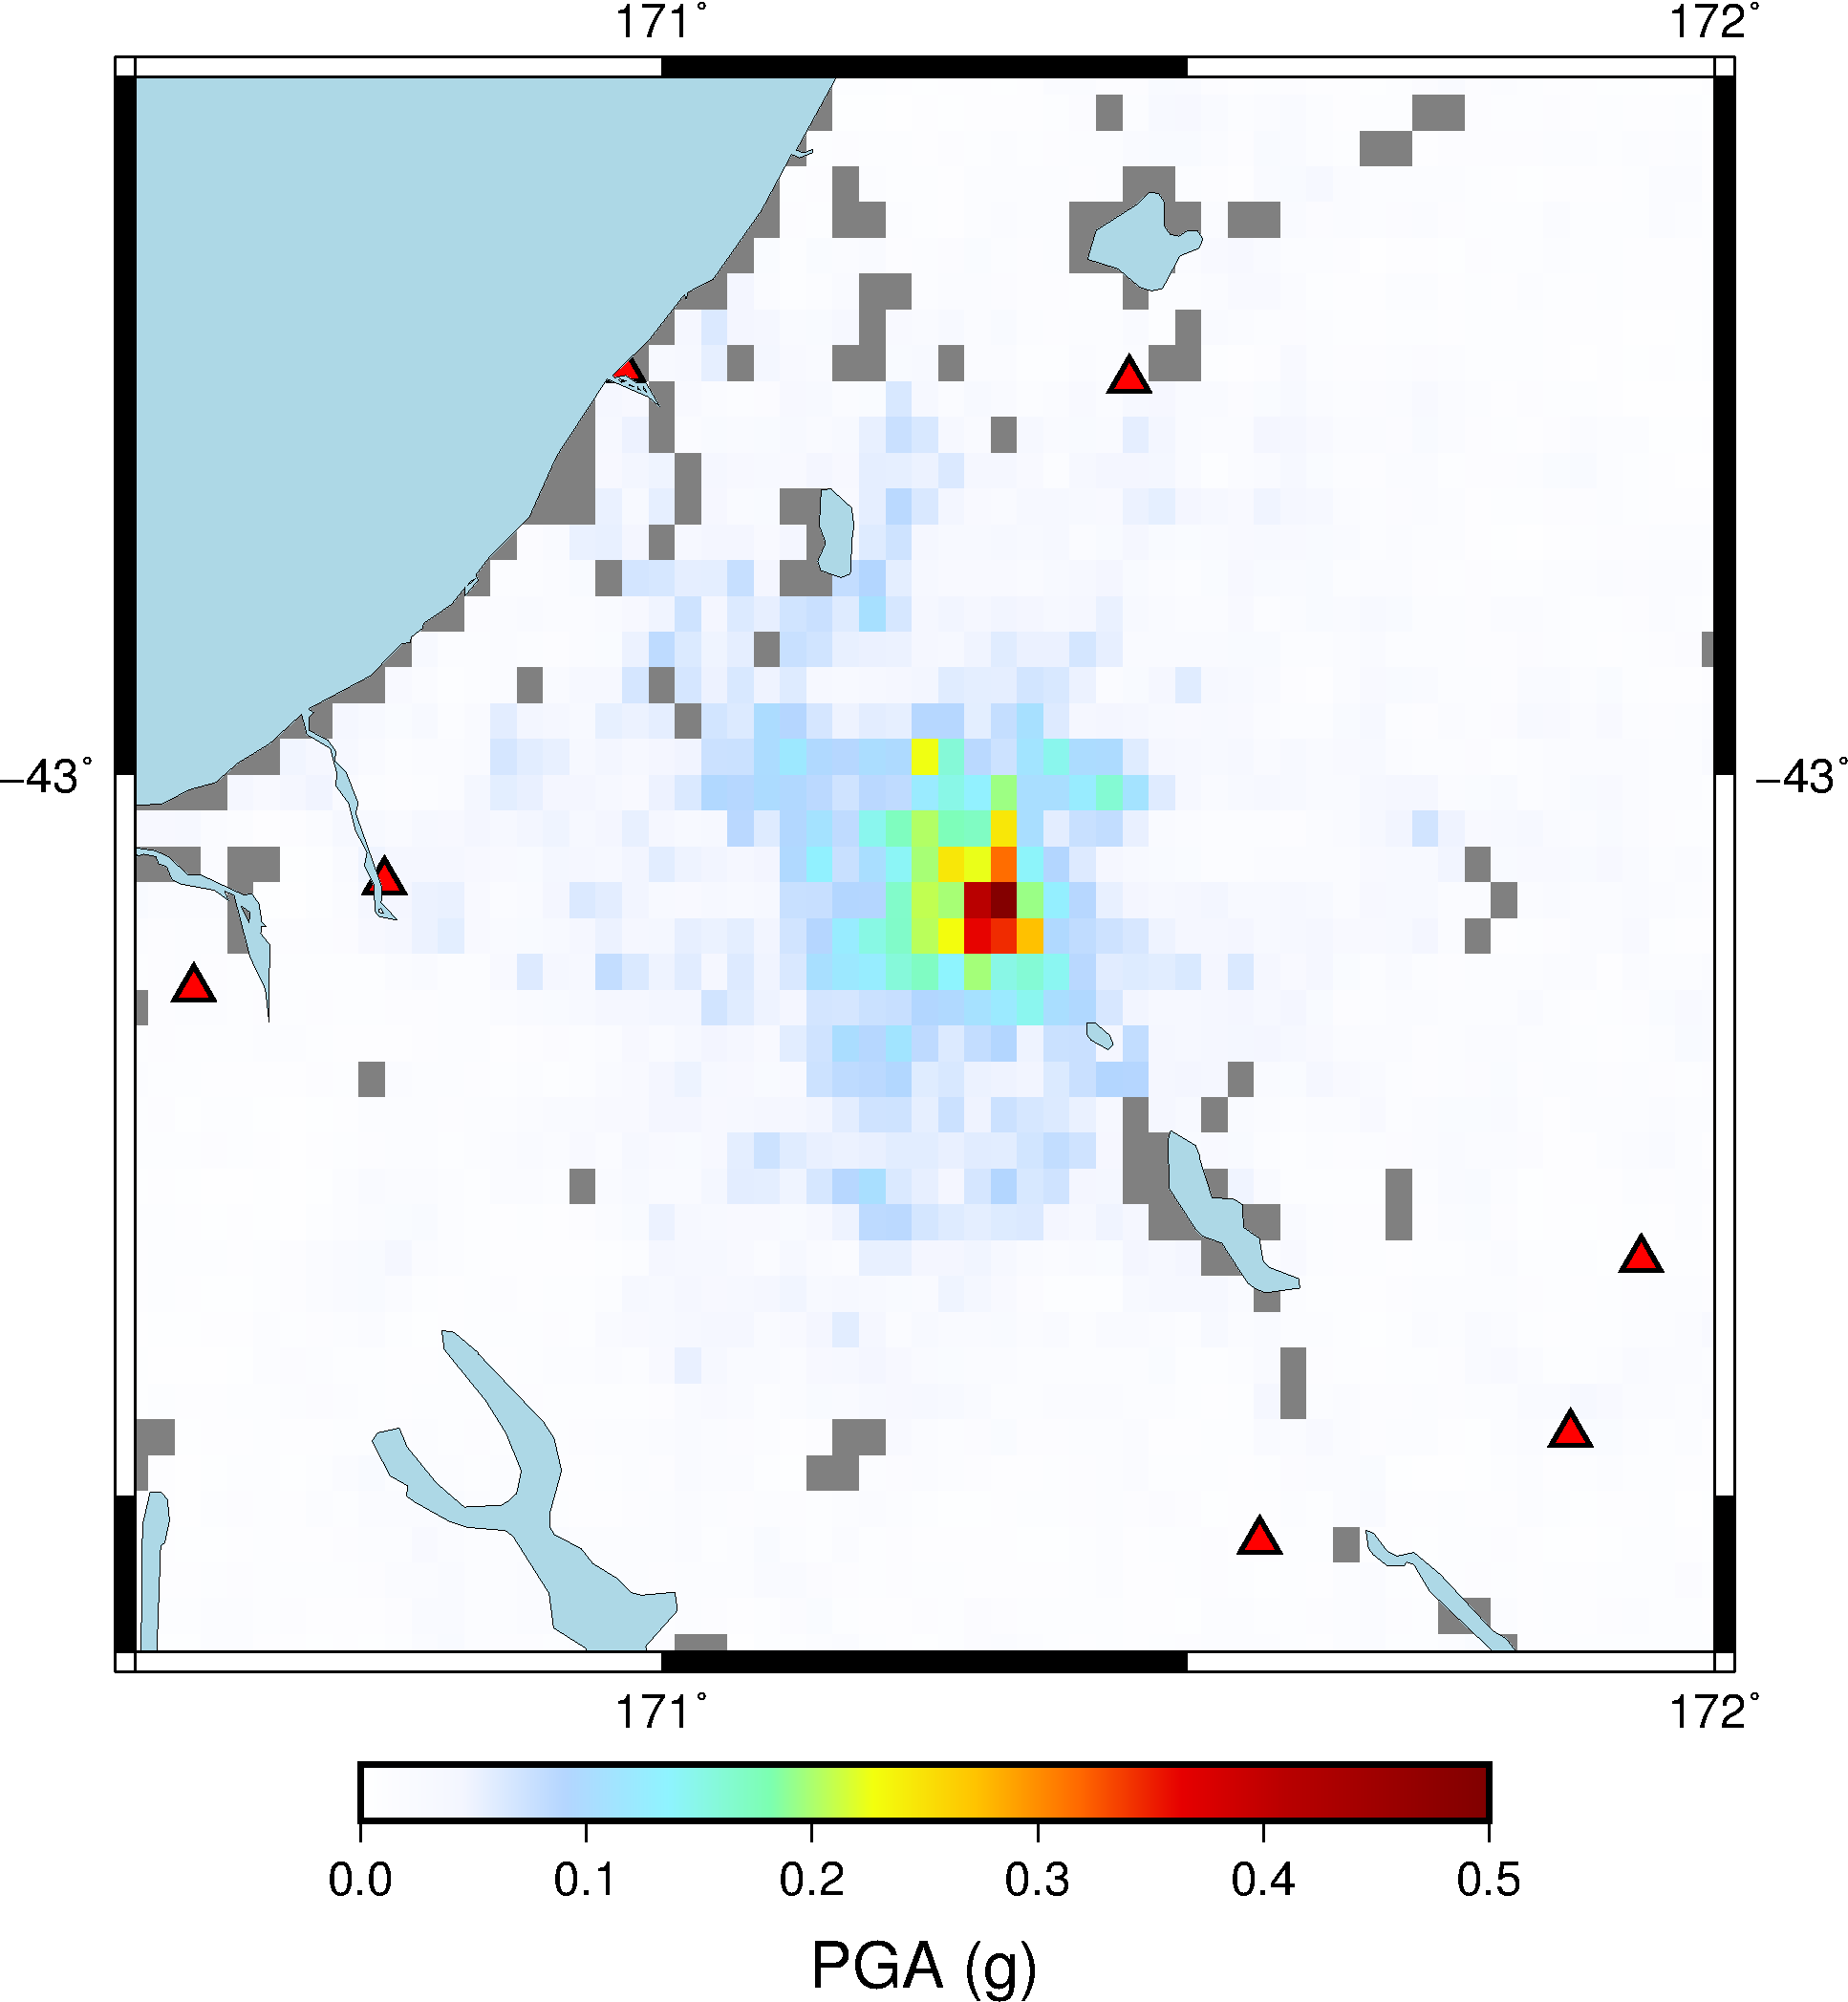
\includegraphics[width = 3in]{GMF_1b.png}}
\subfloat[d]{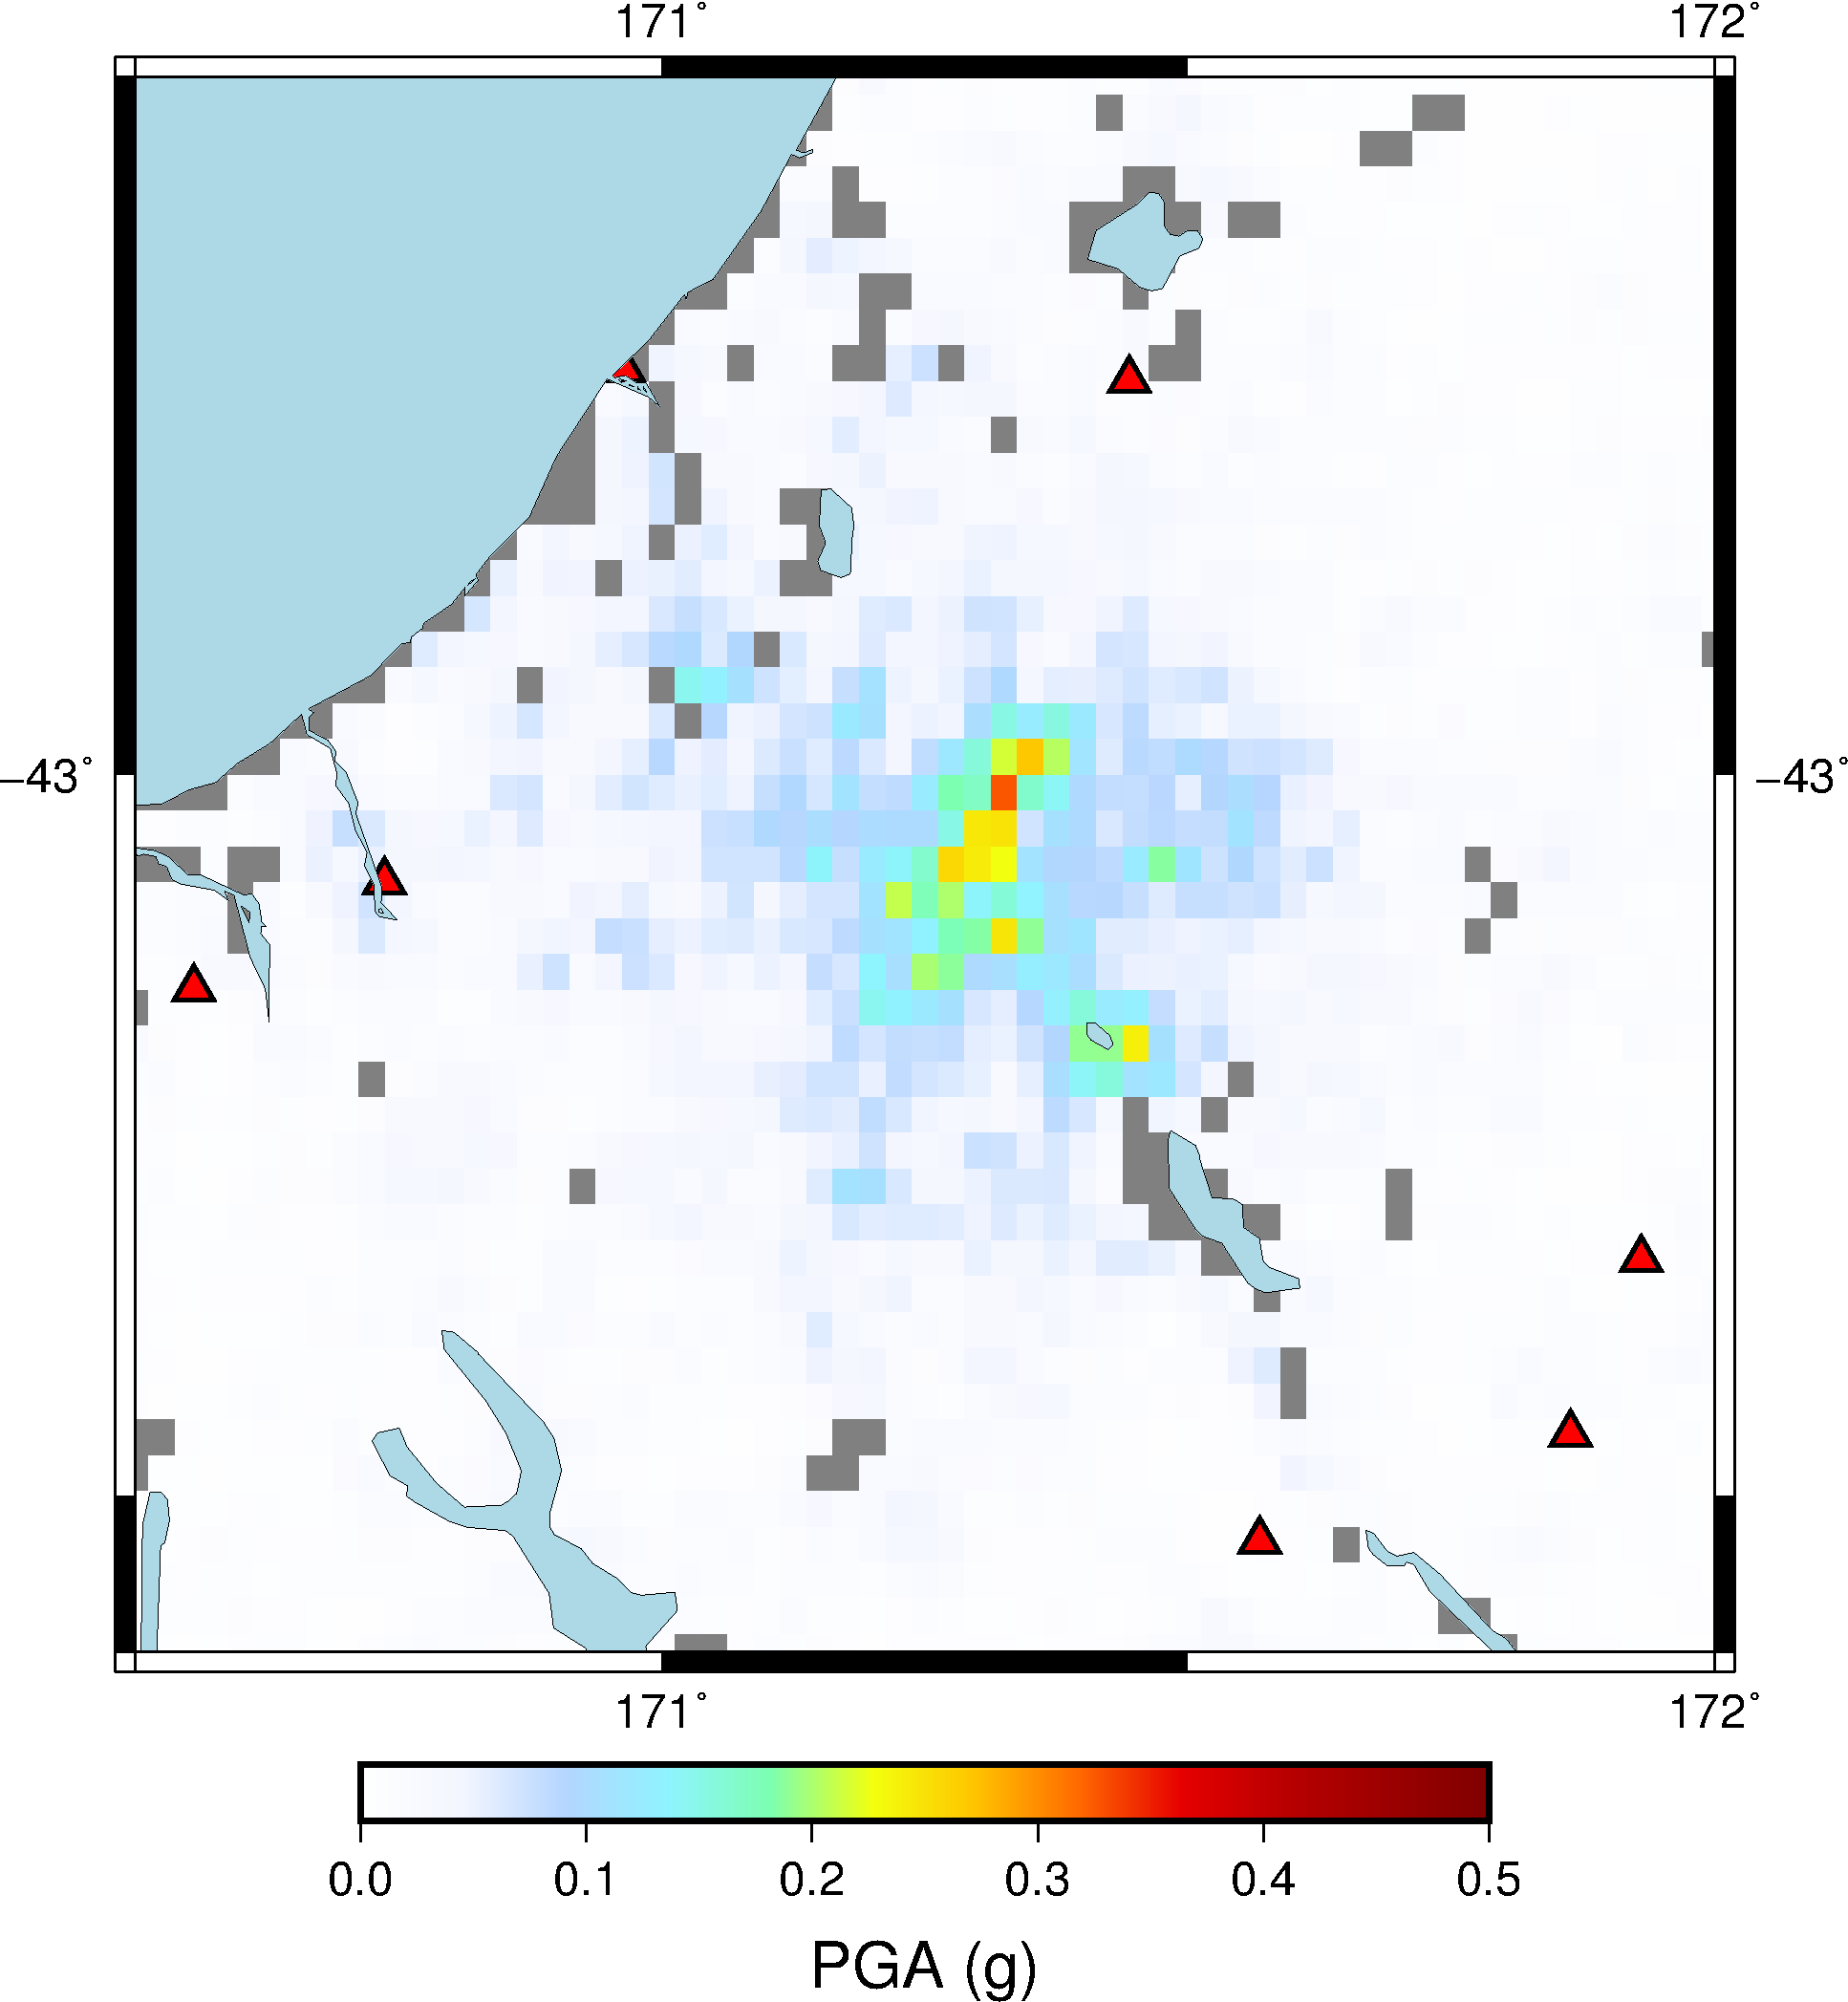
\includegraphics[width = 3in]{GMF_1c.png}} 
\caption{Ground motion simulations of spatially correlated residuals conditional on observed data. A) Median ShakeMap, B-D) Three different realisations of a ground motion field}
\label{gmfs}
\end{figure}

\begin{thebibliography}{9}

\bibitem{park2007}
  J. Park and P. Bazzurro and J. Baker,
  \emph{Modeling spatial correlation of ground motion intensity measures for regional seismic hazard and portfolio loss estimation}.
  Applications of statistics and probability in civil engineering, Kanada, Takada and Furuta (ends),
  Taylor and Francis Group London, ISBN 978-0-415-45211-3,
  2007.

\end{thebibliography}

\end{document}  